% Source: AESP_466_ClassWork/Supplements/Notes/latex/6.2.4/6.2.4.tex

\documentclass[border=4pt]{standalone}
\usepackage{amsmath,amssymb,amsthm}
\usepackage{graphicx}
\usepackage{tikz}
\usepackage{xcolor}
\usetikzlibrary{arrows.meta,calc,positioning,decorations.markings,patterns,shapes.geometric,angles,quotes}

\definecolor{Garnet}{HTML}{73000A}
\definecolor{USC_Rose}{HTML}{CC2E40}
\definecolor{USC_Blue}{HTML}{466A9F}
\definecolor{USC_Slate}{HTML}{1F414D}
\definecolor{USC_Olive}{HTML}{65780B}
\definecolor{USC_Lime}{HTML}{CED318}
\definecolor{USC_Gold}{HTML}{A49137}
\definecolor{USC_Black90}{HTML}{565556}
\definecolor{USC_Black10}{HTML}{ECECEC}

\newcommand{\vect}[1]{\mathbf{#1}}
\newcommand{\mat}[1]{\mathbf{#1}}
\newcommand{\uvec}[1]{\hat{\mathbf{#1}}}
\newcommand{\transpose}{^{\mkern-1.5mu\mathsf{T}}}
\newcommand{\inv}{^{-1}}
\newcommand{\deriv}[2]{\frac{d #1}{d #2}}
\newcommand{\pderiv}[2]{\frac{\partial #1}{\partial #2}}

\begin{document}
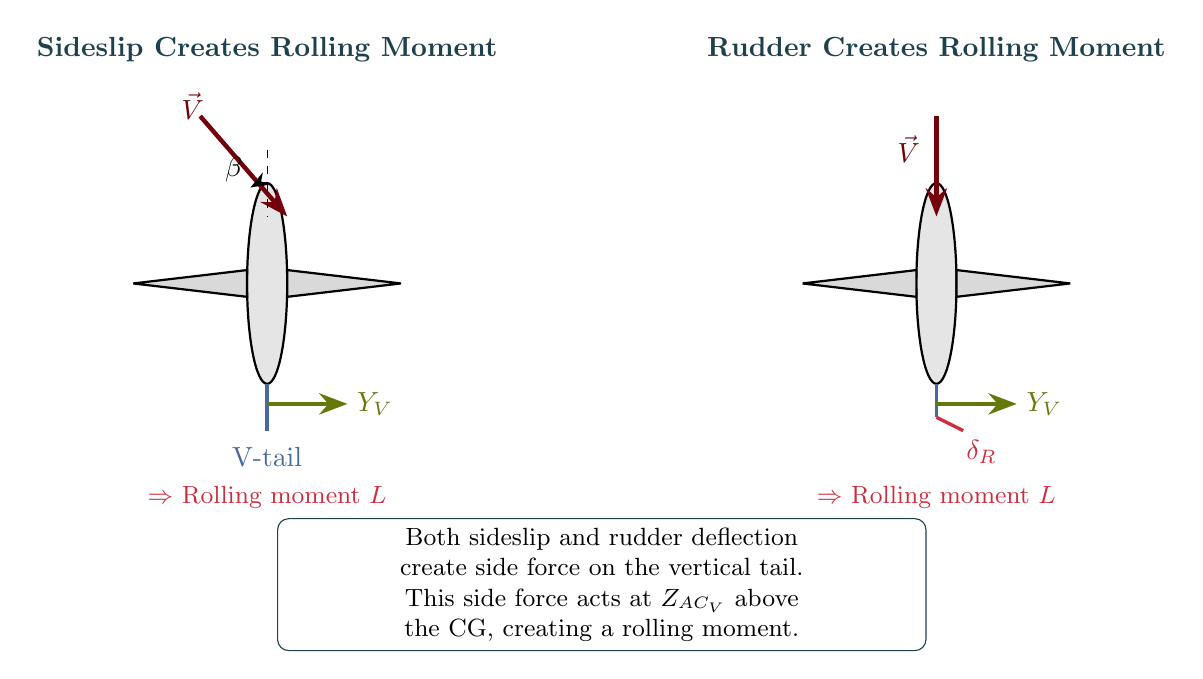
\begin{tikzpicture}[>=Stealth, scale=0.85]
    % Left panel: Sideslip case
    \begin{scope}[shift={(-5,0)}]
        % Title
        \node[font=\bfseries, USC_Slate] at (0,3.5) {Sideslip Creates Rolling Moment};

        % Aircraft top view (simplified)
        \draw[thick, fill=gray!20] (0,0) ellipse (0.3 and 1.5);

        % Wings
        \draw[thick, fill=gray!30] (-2,0) -- (-0.3,0.2) -- (-0.3,-0.2) -- (-2,0);
        \draw[thick, fill=gray!30] (2,0) -- (0.3,0.2) -- (0.3,-0.2) -- (2,0);

        % Vertical tail (top view - just a line)
        \draw[very thick, USC_Blue] (0,-1.5) -- (0,-2.2);
        \node[USC_Blue, below] at (0,-2.3) {V-tail};

        % Velocity vector (at angle showing sideslip)
        \draw[->, ultra thick, Garnet] (-1,2.5) -- (0.3,1);
        \node[Garnet, above left] at (-0.8,2.3) {$\vec{V}$};

        % Sideslip angle
        \draw[dashed] (0,2) -- (0,1);
        \draw[->, thick] (0,1.5) arc (90:120:0.5);
        \node at (-0.5,1.7) {$\beta$};

        % Side force on tail
        \draw[->, ultra thick, USC_Olive] (0,-1.8) -- (1.2,-1.8);
        \node[USC_Olive, right] at (1.2,-1.8) {$Y_V$};

        % Rolling moment indication
        \node[USC_Rose, font=\small] at (0,-3.2) {$\Rightarrow$ Rolling moment $L$};
    \end{scope}

    % Right panel: Rudder case
    \begin{scope}[shift={(5,0)}]
        % Title
        \node[font=\bfseries, USC_Slate] at (0,3.5) {Rudder Creates Rolling Moment};

        % Aircraft top view (simplified)
        \draw[thick, fill=gray!20] (0,0) ellipse (0.3 and 1.5);

        % Wings
        \draw[thick, fill=gray!30] (-2,0) -- (-0.3,0.2) -- (-0.3,-0.2) -- (-2,0);
        \draw[thick, fill=gray!30] (2,0) -- (0.3,0.2) -- (0.3,-0.2) -- (2,0);

        % Vertical tail with rudder deflected
        \draw[very thick, USC_Blue] (0,-1.5) -- (0,-2.0);
        \draw[very thick, USC_Rose] (0,-2.0) -- (0.4,-2.2);
        \node[USC_Rose, below right] at (0.3,-2.2) {$\delta_R$};

        % Velocity vector (straight)
        \draw[->, ultra thick, Garnet] (0,2.5) -- (0,1);
        \node[Garnet, left] at (-0.1,2) {$\vec{V}$};

        % Side force on tail
        \draw[->, ultra thick, USC_Olive] (0,-1.8) -- (1.2,-1.8);
        \node[USC_Olive, right] at (1.2,-1.8) {$Y_V$};

        % Rolling moment indication
        \node[USC_Rose, font=\small] at (0,-3.2) {$\Rightarrow$ Rolling moment $L$};
    \end{scope}

    % Connecting explanation
    \node[draw=USC_Slate, fill=white, rounded corners, align=center, font=\small, text width=8cm] at (0,-4.5) {
        Both sideslip and rudder deflection create side force on the vertical tail.\\
        This side force acts at $Z_{AC_V}$ above the CG, creating a rolling moment.
    };

\end{tikzpicture}
\end{document}
